% AAAI-Style Two-Column Format (Custom Implementation)
% This uses standard packages to achieve AAAI-like formatting

\documentclass[letterpaper]{article}

% AAAI-like formatting
\usepackage[margin=1.75cm, top=2cm, bottom=2cm]{geometry}
\usepackage{times}
\usepackage{helvet}
\usepackage{courier}
\usepackage[hyphens]{url}
\usepackage{graphicx}
\urlstyle{rm}
\def\UrlFont{\rm}
\usepackage{natbib}
\usepackage{caption}
\frenchspacing
\setlength{\pdfpagewidth}{8.5in}
\setlength{\pdfpageheight}{11in}

% Two-column layout
\usepackage{multicol}
\setlength{\columnsep}{0.5cm}

% Additional packages
\usepackage{amsmath,amssymb,amsfonts}
\usepackage{booktabs}
\usepackage{multirow}
\usepackage{tikz}
\usetikzlibrary{shapes,arrows.meta,positioning,fit,calc}
\usepackage{float}
\usepackage{hyperref}

% Title formatting (AAAI-like)
\makeatletter
\renewcommand{\maketitle}{%
  \begin{center}
    {\Large\bfseries \@title \par}
    \vspace{1em}
    {\normalsize \@author \par}
    \vspace{1.5em}
  \end{center}
}
\makeatother

% Section formatting
\usepackage{titlesec}
\titleformat{\section}{\normalfont\bfseries}{\thesection}{1em}{}
\titleformat{\subsection}{\normalfont\bfseries}{\thesubsection}{1em}{}
\titleformat{\subsubsection}{\normalfont\itshape}{\thesubsubsection}{1em}{}

\setcounter{secnumdepth}{2}

\title{Partisan Discourse on X: An Analysis of Political Polarization in Social Media}

\author{
Ziv Barretto, Agriya Yadav, Kyra Chhetri, Anirban Sen\\
Ashoka University
}

\begin{document}

\maketitle

\begin{multicols}{2}

\begin{abstract}
This paper investigates partisan discourse on X (formerly Twitter), examining how political identities and affiliations shape online communication patterns. We analyze a large-scale dataset of tweets retweeted by Indian politicians from 2020-2023 to understand political polarization in social media. Our methodology combines influencer polarity scoring based on retweet behavior, automated keyword extraction using KeyBERT, and stance classification using a LoRA-adapted large language model. We identify politically polar keywords and classify tweet stances toward these topics to reveal patterns in how ruling and opposition parties engage with different political narratives.
\end{abstract}

\section{Introduction}

The rise of social media platforms has fundamentally transformed political communication and discourse. X (formerly known as Twitter) has emerged as a critical platform for political discussion, serving as a space where politicians, journalists, activists, and citizens engage in real-time conversations about political issues. However, this democratization of political discourse has coincided with growing concerns about political polarization and the formation of ideological echo chambers.

This paper investigates partisan discourse on X, examining how political identities and affiliations shape online communication patterns. We focus on the Indian political context, analyzing how politicians from ruling and opposition parties engage with content from various influencers and how this engagement reflects broader patterns of political polarization.

\section{Literature Review}

% TODO: Add literature review content

\section{Data Collection}

\subsection{Data Source}

We utilize a dataset of tweets provided by Professor Joyojeet Pal, comprising retweets made by Indian politicians on X (Twitter) during the period 2020--2023. The dataset contains over 7.1 million retweet records, capturing the amplification behavior of politicians across the Indian political spectrum. Each record represents a retweet action, containing: (1) the original tweet content, (2) the timestamp, (3) the retweeting politician's X handle, and (4) the original author (influencer) whose content was retweeted.

\subsection{Political Affiliation Mapping}

To associate politicians with their party affiliations, we utilize an external mapping file containing X handles and corresponding party memberships. This mapping covers politicians from over 50 political parties, which we aggregate into two major blocs for analysis:

\begin{itemize}
    \item \textbf{Ruling Bloc}: BJP, JDU, LJP, HAM, JSP, NPP, AIADMK, AJSU, AGP, RPI, NPF, IPFT, NDPP, RSS, NDA, MNF, VHP, YSRCP, ABVP, BJD, BSCP, and affiliated parties
    \item \textbf{Opposition Bloc}: INC, AITC/TMC, DMK, SP, CPIM, RJD, AAP, JMM, IUML, CPI, NCP, TRS, Shiv Sena, TDP, JDS, and allied parties
\end{itemize}

\subsection{Data Processing Pipeline}

The data processing consists of two major stages:

\subsubsection{Stage 1: Party Labeling}
We process the raw combined CSV in chunks (100,000 rows per batch) and match each retweeting politician's handle to their party affiliation using lowercase normalization. This produces the labeled dataset with the \texttt{retweet\_party} column populated.

\subsubsection{Stage 2: Polarity Calculation}
For each influencer (original tweet author), we compute yearly polarity scores based on who retweets their content, then average across years to obtain a stable polarity measure. This process identifies 960 unique influencers with calculable polarity scores.

\subsection{Dataset Statistics}

Table~\ref{tab:dataset_stats} presents the key statistics of our raw and processed datasets.

\vspace{0.5em}
\begin{center}
\small
\captionof{table}{Dataset Statistics}
\label{tab:dataset_stats}
\begin{tabular}{lr}
\toprule
\textbf{Metric} & \textbf{Value} \\
\midrule
Total retweets & 7,115,963 \\
English tweets & 2,939,716 (41.3\%) \\
Hindi/Regional tweets & 4,176,247 (58.7\%) \\
Unique influencers (with polarity) & 960 \\
Influencer-year observations & 3,712 \\
Temporal range & 2020--2023 \\
\bottomrule
\end{tabular}
\end{center}
\vspace{0.5em}

The temporal distribution of tweets, shown in Table~\ref{tab:temporal_dist}, indicates activity across all four years, with 2021 showing the highest volume.

\vspace{0.5em}
\begin{center}
\small
\captionof{table}{Temporal Distribution of Tweets}
\label{tab:temporal_dist}
\begin{tabular}{lrr}
\toprule
\textbf{Year} & \textbf{Influencer-Year Records} \\
\midrule
2020 & 908 \\
2021 & 944 \\
2022 & 949 \\
2023 & 911 \\
\bottomrule
\end{tabular}
\end{center}
\vspace{0.5em}

\subsection{Data Structure}

Table~\ref{tab:columns} describes the key columns in our final processed dataset.

\vspace{0.5em}
\begin{center}
\footnotesize
\captionof{table}{Dataset Column Descriptions}
\label{tab:columns}
\begin{tabular}{p{2.2cm}p{4.3cm}}
\toprule
\textbf{Column} & \textbf{Description} \\
\midrule
\texttt{timestamp} & Date and time of the retweet (UTC) \\
\texttt{tweet} & Full text content of original tweet \\
\texttt{retweet\_author} & X handle of retweeting politician \\
\texttt{original\_author} & X handle of influencer \\
\texttt{retweet\_party} & Political party of retweeter \\
\texttt{year} & Year extracted from timestamp \\
\texttt{side} & Political bloc (ruling/opposition/other) \\
\texttt{polarity\_avg} & Influencer's average polarity score \\
\texttt{tweet\_label} & Inferred political leaning of tweet \\
\bottomrule
\end{tabular}
\end{center}
\vspace{0.5em}

\subsection{English Language Filtering}

The original dataset contains tweets in multiple languages, including Hindi and regional Indian languages. For the English analysis pipeline, we filter tweets using an ASCII-ratio heuristic: a tweet is classified as English if at least 85\% of its alphabetic characters are ASCII letters. This approach is computationally efficient for large-scale processing while maintaining reasonable accuracy for language detection.

\section{Methodology}

\subsection{Influencer Polarity Calculation}

A key insight of our approach is that politicians' retweet behavior reveals their political alignments. When a politician retweets content from an external account (influencer), it signals endorsement or amplification of that content. By aggregating retweet patterns across many politicians with known party affiliations, we can infer the political leaning of influencers.

\subsubsection{Polarity Score Formulation}

We first map all political parties to two major blocs: \textit{Ruling} (e.g., BJP, NDA coalition partners) and \textit{Opposition} (e.g., INC, TMC, AAP, and other INDIA bloc parties). For each influencer $i$ and year $y$, we calculate a yearly polarity score:

\begin{equation}
P_{i,y} = \frac{R_{i,y} - O_{i,y}}{R_{i,y} + O_{i,y}}
\label{eq:polarity}
\end{equation}

\noindent where $R_{i,y}$ is the count of retweets the influencer received from Ruling bloc politicians in year $y$, and $O_{i,y}$ is the count from Opposition bloc politicians.

The polarity score ranges from $-1$ (exclusively retweeted by Opposition) to $+1$ (exclusively retweeted by Ruling). We then compute an average polarity score across all available years for each influencer:

\begin{equation}
P_{avg,i} = \frac{1}{|Y_i|} \sum_{y \in Y_i} P_{i,y}
\end{equation}

\noindent where $Y_i$ is the set of years in which influencer $i$ was retweeted.

\subsubsection{Classification Thresholds}

Based on the average polarity score, influencers are classified into three categories:

\begin{itemize}
    \item \textbf{Pro-Ruling}: $P_{avg} \geq 0.5$
    \item \textbf{Pro-Opposition}: $P_{avg} \leq -0.5$
    \item \textbf{Neutral}: $-0.5 < P_{avg} < 0.5$
\end{itemize}

This classification is then propagated to all tweets authored by each influencer, labeling tweets based on the political leaning of their author.

\subsubsection{Justification for This Approach}

Alternative approaches to measuring political polarity include:
\begin{itemize}
    \item \textbf{Hashtag-based}: Inferring polarity from hashtag usage. However, hashtags can be appropriated, used sarcastically, or vary in political signal strength.
    \item \textbf{Content-based}: Using sentiment analysis on tweet text. These methods struggle with context, sarcasm, and nuanced political language.
    \item \textbf{Network-based}: Analyzing follower/following relationships. These are more stable but require extensive social graph data.
\end{itemize}

Our retweet-based approach leverages the revealed preferences of politicians---a retweet represents an explicit endorsement action, providing a more reliable signal than passive following or hashtag co-occurrence.

\subsection{Keyword Extraction with KeyBERT}

To identify the topics discussed in partisan discourse, we employ KeyBERT for automated keyword extraction from tweet text.

\subsubsection{KeyBERT Methodology}

KeyBERT uses sentence-level embeddings to identify keywords and phrases that are semantically similar to the document as a whole. The algorithm:

\begin{enumerate}
    \item Encodes the input document using a Sentence-BERT model
    \item Generates candidate keywords/phrases
    \item Encodes each candidate into the same embedding space
    \item Ranks candidates by cosine similarity
    \item Applies Maximal Marginal Relevance (MMR) for diversity
\end{enumerate}

\subsubsection{Configuration}

We use the following configuration:

\begin{itemize}
    \item \textbf{Model}: \texttt{paraphrase-multilingual-MiniLM-L12-v2}
    \item \textbf{N-gram range}: 1--2 (unigrams and bigrams)
    \item \textbf{Top-N}: 3 keywords per tweet
    \item \textbf{Diversity}: 0.7 (MMR parameter)
\end{itemize}

\subsubsection{Preprocessing}

Before keyword extraction, tweets undergo preprocessing: URL removal, mention extraction (@ handles converted to tokens), hashtag segmentation (e.g., \texttt{\#AatmaNirbharBharat} $\rightarrow$ ``aatma nirbhar bharat''), and whitespace normalization.

\subsubsection{Polar Keyword Selection}

After extracting keywords from all tweets, we identify \textit{polar keywords}---topics that are disproportionately discussed by one political side. Keyword polarity is determined by analyzing the proportion of tweets from Pro-Ruling versus Pro-Opposition sources for each keyword.

\paragraph{Initial Keyword Set (15 Keywords)}
We first selected 15 keywords representing major political topics for manual annotation. These keywords were chosen based on their political significance and representation across both ruling and opposition discourse. Table~\ref{tab:polar_keywords} presents these keywords.

\vspace{0.5em}
\begin{center}
\footnotesize
\captionof{table}{Initial 15 Keywords for Manual Annotation}
\label{tab:polar_keywords}
\begin{tabular}{lp{2cm}}
\toprule
\textbf{Keyword} & \textbf{Dominant Side} \\
\midrule
caa & Pro-Opposition \\
china & Mixed \\
congress & Pro-Ruling \\
farm\_laws & Pro-Opposition \\
farmers\_protests & Pro-Opposition \\
hindu & Pro-Ruling \\
hindutva & Pro-Opposition \\
kashmir & Mixed \\
kashmiri\_pandits & Pro-Ruling \\
modi & Pro-Ruling \\
muslim & Pro-Opposition \\
new\_parliament & Pro-Ruling \\
rahulgandhi & Mixed \\
ram\_mandir & Pro-Ruling \\
shaheen\_bagh & Pro-Opposition \\
\bottomrule
\end{tabular}
\end{center}
\vspace{0.5em}

\paragraph{Extended Keyword Set (23 Additional Keywords)}
To expand coverage, we identified 23 additional polar keywords by analyzing tweet counts for each political bloc. Keywords were selected based on (1) clear partisan skew in usage patterns, and (2) relevance to significant political events or narratives. Table~\ref{tab:extended_keywords} presents a sample of these additional keywords with their extraction statistics.

\vspace{0.5em}
\begin{center}
\footnotesize
\captionof{table}{Sample Extended Polar Keywords with Extraction Stats}
\label{tab:extended_keywords}
\begin{tabular}{lrrr}
\toprule
\textbf{Keyword} & \textbf{Total} & \textbf{Pro-Ruling} & \textbf{Pro-Opp} \\
\midrule
ucc & 7,738 & 5,690 (74\%) & 2,048 \\
democracy & 7,612 & 2,981 (39\%) & 4,631 \\
mahotsav & 5,455 & 5,361 (98\%) & 94 \\
aatmanirbhar & 5,386 & 5,289 (98\%) & 97 \\
msp & 5,567 & 3,227 (58\%) & 2,340 \\
sangh & 4,498 & 1,761 (39\%) & 2,737 \\
ayodhya & 2,452 & 1,921 (78\%) & 531 \\
unemployment & 1,649 & 284 (17\%) & 1,365 \\
islamists & 1,488 & 1,470 (99\%) & 18 \\
bhakts & 1,886 & 363 (19\%) & 1,523 \\
\bottomrule
\end{tabular}
\end{center}
\vspace{0.5em}

The extended set includes keywords like \textit{aatmanirbhar} (self-reliance campaign), \textit{ucc} (Uniform Civil Code), \textit{ayodhya}, and \textit{mahotsav} which are predominantly used by Pro-Ruling sources (>74\%), while keywords like \textit{unemployment}, \textit{demonetisation}, \textit{bhakts}, and \textit{spyware} are predominantly discussed by Pro-Opposition sources (>80\%).

\subsection{Stance Classification}

To understand how different political factions discuss polar topics, we develop a stance classification system that determines whether a tweet expresses support, opposition, or neutrality toward a given keyword/entity.

\subsubsection{Problem Formulation}

Given a tweet $t$ and a target entity (keyword) $e$, the stance classification task predicts one of three labels:
\begin{itemize}
    \item \textbf{Favor}: Support for the entity
    \item \textbf{Against}: Opposition to the entity
    \item \textbf{Neutral}: No clear positive/negative stance
\end{itemize}

\subsubsection{Model Architecture}

We employ a large language model (LLM) adapted for stance classification:

\begin{itemize}
    \item \textbf{Base Model}: Mistral-7B-Instruct, a 7-billion parameter instruction-tuned language model
    \item \textbf{Adaptation}: Low-Rank Adaptation (LoRA), which freezes pre-trained weights and injects trainable rank decomposition matrices
\end{itemize}

LoRA enables parameter-efficient fine-tuning by decomposing weight updates into low-rank matrices:

\begin{equation}
W' = W + BA
\end{equation}

\noindent where $W$ is the frozen pre-trained weight matrix, and $B \in \mathbb{R}^{d \times r}$, $A \in \mathbb{R}^{r \times k}$ are trainable low-rank matrices with rank $r \ll \min(d, k)$.

\subsubsection{Manual Annotation Process}

For the initial 15 keywords, we manually annotated tweets to create training and evaluation data:

\begin{enumerate}
    \item \textbf{Sampling}: For each keyword, we sampled 100--150 tweets, balancing Pro-Ruling and Pro-Opposition sources
    \item \textbf{Deduplication}: Removed duplicate tweets and near-duplicates to ensure annotation quality
    \item \textbf{Labeling}: Each tweet was labeled with stance (favor/against/neutral) and a brief reasoning
    \item \textbf{Consolidation}: Annotations were organized into per-keyword files
\end{enumerate}

The final annotated dataset comprises 1,866 labeled tweet-keyword pairs across 15 keywords.

\subsubsection{Training and Evaluation Split}

The annotated data was split 85:15 for training few-shot examples and held-out evaluation, using stratified sampling to maintain class balance across keywords.

\begin{itemize}
    \item \textbf{Training set}: 10 examples per keyword (3 favor, 3 against, 3 neutral, 1 filler) used as few-shot prompts
    \item \textbf{Test set}: 264 samples for evaluation
\end{itemize}

\subsubsection{Few-Shot Inference}

During inference, the system dynamically retrieves keyword-specific few-shot examples to construct the prompt. If keyword-specific examples are unavailable (for the extended 23 keywords), the system falls back to a global set of examples, enabling stance classification across all 38 keywords.

\subsubsection{Output Format}

The model generates structured JSON output:

\begin{verbatim}
{
  "stance": "favor|against|neutral",
  "reason": "<brief explanation>"
}
\end{verbatim}

\subsubsection{Model Evaluation}

We evaluated the LoRA-adapted model on the held-out test set of 264 samples. Table~\ref{tab:eval_overall} presents the overall classification performance.

\vspace{0.5em}
\begin{center}
\footnotesize
\captionof{table}{Stance Classification Evaluation Results}
\label{tab:eval_overall}
\begin{tabular}{lr}
\toprule
\textbf{Metric} & \textbf{Value} \\
\midrule
Total test samples & 264 \\
Accuracy & 78.0\% \\
Precision (macro) & 78.0\% \\
Recall (macro) & 75.3\% \\
F1-Score (macro) & 76.2\% \\
F1-Score (weighted) & 77.7\% \\
\bottomrule
\end{tabular}
\end{center}
\vspace{0.5em}

Table~\ref{tab:eval_perclass} shows the per-class performance breakdown.

\vspace{0.5em}
\begin{center}
\footnotesize
\captionof{table}{Per-Class Classification Performance}
\label{tab:eval_perclass}
\begin{tabular}{lrrrr}
\toprule
\textbf{Class} & \textbf{Precision} & \textbf{Recall} & \textbf{F1} & \textbf{Support} \\
\midrule
Against & 0.78 & 0.80 & 0.79 & 95 \\
Favor & 0.78 & 0.86 & 0.82 & 111 \\
Neutral & 0.78 & 0.60 & 0.68 & 58 \\
\bottomrule
\end{tabular}
\end{center}
\vspace{0.5em}

The model achieves strongest performance on the ``favor'' class (F1=0.82), followed by ``against'' (F1=0.79). The ``neutral'' class shows lower recall (0.60), reflecting the inherent difficulty in distinguishing neutral stances from weakly expressed opinions.

Table~\ref{tab:eval_keyword} presents per-keyword accuracy, showing variation across different political topics.

\vspace{0.5em}
\begin{center}
\footnotesize
\captionof{table}{Per-Keyword Classification Accuracy (Top 10)}
\label{tab:eval_keyword}
\begin{tabular}{lrr}
\toprule
\textbf{Keyword} & \textbf{Accuracy} & \textbf{F1 (macro)} \\
\midrule
modi & 94.4\% & 0.91 \\
caa & 89.5\% & 0.90 \\
congress & 88.9\% & 0.84 \\
hindutva & 85.7\% & 0.56 \\
new\_parliament & 85.7\% & 0.82 \\
rahulgandhi & 81.3\% & 0.81 \\
farmers\_protests & 80.0\% & 0.82 \\
shaheen\_bagh & 78.9\% & 0.71 \\
muslim & 78.9\% & 0.79 \\
china & 73.7\% & 0.64 \\
\bottomrule
\end{tabular}
\end{center}
\vspace{0.5em}


\subsection{Hindi Tweet Analysis Pipeline}

For analyzing Hindi-language tweets, we extend the stance classification pipeline:

\subsubsection{Multilingual Model Support}

The Mistral-7B model supports multilingual input, enabling direct processing of Hindi tweets. The few-shot examples for Hindi tweets are constructed with Hindi text while maintaining the same JSON output format.

\subsubsection{Fallback Mechanism}

The pipeline implements hierarchical few-shot example retrieval:
\begin{enumerate}
    \item Attempt to load keyword-specific examples
    \item If unavailable, fall back to a global fallback JSON
\end{enumerate}

This ensures robust inference even for keywords without dedicated few-shot examples.

\vspace{0.5em}
\begin{center}
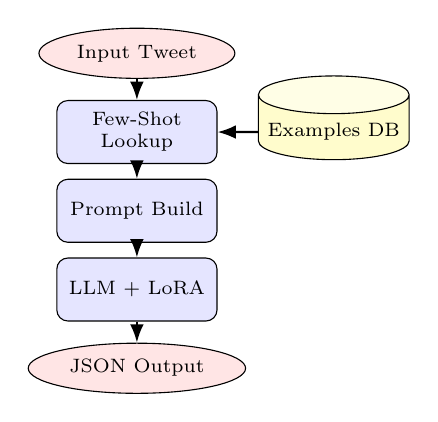
\begin{tikzpicture}[
    node distance=1cm,
    auto,
    block/.style={
        rectangle,
        draw,
        fill=blue!10,
        text width=1.8cm,
        text centered,
        rounded corners,
        minimum height=0.8cm,
        font=\scriptsize
    },
    cloud/.style={
        draw,
        ellipse,
        fill=red!10,
        minimum height=0.6cm,
        font=\scriptsize
    },
    database/.style={
        cylinder,
        cylinder uses custom fill,
        cylinder body fill=yellow!20,
        cylinder end fill=yellow!10,
        shape border rotate=90,
        draw,
        aspect=0.25,
        minimum height=1cm,
        text centered,
        font=\scriptsize
    },
    line/.style={
        draw,
        -Latex,
        thick
    }
]

% Nodes
\node [cloud] (input) {Input Tweet};
\node [block, below of=input] (lookup) {Few-Shot Lookup};
\node [database, right of=lookup, node distance=2.5cm] (db) {Examples DB};
\node [block, below of=lookup] (prompt) {Prompt Build};
\node [block, below of=prompt] (llm) {LLM + LoRA};
\node [cloud, below of=llm] (output) {JSON Output};

% Edges
\path [line] (input) -- (lookup);
\path [line] (db) -- (lookup);
\path [line] (lookup) -- (prompt);
\path [line] (prompt) -- (llm);
\path [line] (llm) -- (output);

\end{tikzpicture}
\captionof{figure}{Stance Detection System Architecture}
\label{fig:architecture}
\end{center}
\vspace{0.5em}


\section{Results}

% TODO: Add results content

\subsection{Partisan Network Structure}

\subsection{Content Characteristics}

\subsection{Interaction Patterns}

\subsection{Temporal Dynamics}

\section{Discussion}

% TODO: Add discussion content

\section{Conclusion}

% TODO: Add conclusion content

\section*{Acknowledgment}

We thank Professor Joyojeet Pal for providing the tweet dataset used in this research, and Ashoka University for supporting this work.

\end{multicols}

\end{document}
